%%
%% This is file `sample-acmlarge.tex',
%% generated with the docstrip utility.
%%
%% The original source files were:
%%
%% samples.dtx  (with options: `acmlarge')
%% 
%% IMPORTANT NOTICE:
%% 
%% For the copyright see the source file.
%% 
%% Any modified versions of this file must be renamed
%% with new filenames distinct from sample-acmlarge.tex.
%% 
%% For distribution of the original source see the terms
%% for copying and modification in the file samples.dtx.
%% 
%% This generated file may be distributed as long as the
%% original source files, as listed above, are part of the
%% same distribution. (The sources need not necessarily be
%% in the same archive or directory.)
%%
%%
%% Commands for TeXCount
%TC:macro \cite [option:text,text]
%TC:macro \citep [option:text,text]
%TC:macro \citet [option:text,text]
%TC:envir table 0 1
%TC:envir table* 0 1
%TC:envir tabular [ignore] word
%TC:envir displaymath 0 word
%TC:envir math 0 word
%TC:envir comment 0 0
%%
%%
%% The first command in your LaTeX source must be the \documentclass
%% command.
%%
%% For submission and review of your manuscript please change the
%% command to \documentclass[manuscript, screen, review]{acmart}.
%%
%% When submitting camera ready or to TAPS, please change the command
%% to \documentclass[sigconf]{acmart} or whichever template is required
%% for your publication.
%%
%%
\documentclass[acmlarge]{acmart}

%%
%% \BibTeX command to typeset BibTeX logo in the docs
\AtBeginDocument{%
  \providecommand\BibTeX{{%
    Bib\TeX}}}

%% Rights management information.  This information is sent to you
%% when you complete the rights form.  These commands have SAMPLE
%% values in them; it is your responsibility as an author to replace
%% the commands and values with those provided to you when you
%% complete the rights form.
\setcopyright{acmcopyright}
\copyrightyear{2018}
\acmYear{2018}
\acmDOI{XXXXXXX.XXXXXXX}


%%
%% These commands are for a JOURNAL article.
\acmJournal{POMACS}
\acmVolume{37}
\acmNumber{4}
\acmArticle{111}
\acmMonth{8}

%%
%% Submission ID.
%% Use this when submitting an article to a sponsored event. You'll
%% receive a unique submission ID from the organizers
%% of the event, and this ID should be used as the parameter to this command.
%%\acmSubmissionID{123-A56-BU3}

%%
%% For managing citations, it is recommended to use bibliography
%% files in BibTeX format.
%%
%% You can then either use BibTeX with the ACM-Reference-Format style,
%% or BibLaTeX with the acmnumeric or acmauthoryear sytles, that include
%% support for advanced citation of software artefact from the
%% biblatex-software package, also separately available on CTAN.
%%
%% Look at the sample-*-biblatex.tex files for templates showcasing
%% the biblatex styles.
%%

%%
%% The majority of ACM publications use numbered citations and
%% references.  The command \citestyle{authoryear} switches to the
%% "author year" style.
%%
%% If you are preparing content for an event
%% sponsored by ACM SIGGRAPH, you must use the "author year" style of
%% citations and references.
%% Uncommenting
%% the next command will enable that style.
%%\citestyle{acmauthoryear}

\usepackage{comment}

%%
%% end of the preamble, start of the body of the document source.
\begin{document}

%%
%% The "title" command has an optional parameter,
%% allowing the author to define a "short title" to be used in page headers.
\title{Model-Centric Federated Machine Learning}

%%
%% The "author" command and its associated commands are used to define
%% the authors and their affiliations.
%% Of note is the shared affiliation of the first two authors, and the
%% "authornote" and "authornotemark" commands
%% used to denote shared contribution to the research.

\author{Authors}
\affiliation{%
  \institution{Institute xx}
  \city{City}
  \country{Country}}
\email{@mail.com}

%%
%% By default, the full list of authors will be used in the page
%% headers. Often, this list is too long, and will overlap
%% other information printed in the page headers. This command allows
%% the author to define a more concise list
%% of authors' names for this purpose.
\renewcommand{\shortauthors}{Trovato et al.}

%%
%% The abstract is a short summary of the work to be presented in the
%% article.
\begin{abstract}
Tranditional Federated Machine Learning follows a server-domincated training paradigm which narrows the application scenarios of federated learning and decreases the enthusiasm of data holders to participate.
\end{abstract}

%%
%% The code below is generated by the tool at http://dl.acm.org/ccs.cfm.
%% Please copy and paste the code instead of the example below.
%%
\begin{CCSXML}
<ccs2012>
 <concept>
  <concept_id>10010520.10010553.10010562</concept_id>
  <concept_desc>Computer systems organization~Embedded systems</concept_desc>
  <concept_significance>500</concept_significance>
 </concept>
 <concept>
  <concept_id>10010520.10010575.10010755</concept_id>
  <concept_desc>Computer systems organization~Redundancy</concept_desc>
  <concept_significance>300</concept_significance>
 </concept>
 <concept>
  <concept_id>10010520.10010553.10010554</concept_id>
  <concept_desc>Computer systems organization~Robotics</concept_desc>
  <concept_significance>100</concept_significance>
 </concept>
 <concept>
  <concept_id>10003033.10003083.10003095</concept_id>
  <concept_desc>Networks~Network reliability</concept_desc>
  <concept_significance>100</concept_significance>
 </concept>
</ccs2012>
\end{CCSXML}

\ccsdesc[500]{Computer systems organization~Embedded systems}
\ccsdesc[300]{Computer systems organization~Redundancy}
\ccsdesc{Computer systems organization~Robotics}
\ccsdesc[100]{Networks~Network reliability}

%%
%% Keywords. The author(s) should pick words that accurately describe
%% the work being presented. Separate the keywords with commas.
\keywords{datasets, neural networks, gaze detection, text tagging}

\received{20 February 2007}
\received[revised]{12 March 2009}
\received[accepted]{5 June 2009}

%%
%% This command processes the author and affiliation and title
%% information and builds the first part of the formatted document.
\maketitle

\section{Introduction}
Introduction:
Federated Learning~\cite{li2020federated}.

\subsection{Related Surveys}
In recent years, federated learning has become a buzzword in various fields, leading to the emergence of numerous FL studies.
These works can be classified into three primary categories: FL systems design, FL appllications and FL toolkits. Extensive surveys are available to summarized the advancement of federated learning, as shown in Table~\ref{table:surveys}.
The initial architectures and concepts for FL systems were summaried by Yang \textit{et al.}~\cite{yang2019federated}. 
They categorize FL into horizontal FL, vertical FL and federated transfer learning based on the distribution characteristics of data, 
which are written in IEEE Standard 3652.1-2020~\cite{yang2021white, IEEEstd3652}. 
Following this, an increasing number of surveys have emerged focusing on enhancing FL system design~\cite{li2020federated,aledhari2020federated, kairouz2021advances, zhang2021survey, li2021survey}. 
From the algorithmic perspective, personlized FL~\cite{kulkarni2020survey, tan2022towards} aims to learn personlized models for each client to address the challenge of statistical heterogeneity~\cite{ma2022state}.
Besides, the privacy-perserving computing platforms and model aggregation protocols for FL systems also been widely studied and sumaried by~\cite{liu2022privacy,el2022differential,yin2021comprehensive,lyu2020threats}.
Furthermore, many advanced FL architectures had been proposed, such as asynchronous~\cite{xu2021asynchronous}, decentralized and blockchain-based FL frameworks~\cite{nguyen2021federated, qu2022blockchain, zhu2022blockchain}.
Given that federated learning technologies enable collaboration among distributed participants in model training and decision-making, this capability holds great promise in a wide range of application scenarios.
For instance, multiple geogrphically distributed medical insitutions can enhace medication recommendation, drug-drug interaction prediction and medical image analysis in a collaborative manner without exchanging any sensitive data~\cite{xu2021federated, pfitzner2021federated, antunes2022federated, rieke2020future}. 
The massive real-time data generated by IoT devices in smart cities~\cite{zhang2022federated, ramu2022federated}, industries~\cite{boopalan2022fusion}, vehicles~\cite{du2020federated} has also sparked interest in exploring how FL technology can be used to deliver more advanced services such as intrusion detection, anomaly detection, fraud detection and network load prediction~\cite{agrawal2022federated, alazab2021federated, ghimire2022recent}.

As summarized in Table~\ref{table:surveys}, most surveys extensively discuss the challenges of efficiency, heterogeneity, privacy in FL systems design, with the surveys from blockchain fileds offering the most comprehensive review.
However, except for a few blockchain-based FL studies, most of the above surveys just present the same story from slightly different angles or backgrounds, i.e a server sets the model training task and delegate it to data holders to complete. 
This \textbf{server-domincated} cooperation framework is a narrow implementation of the FL systems.
Therefore, this survey aim to fill the gap by investigating and surveying the associated tenchnologies that support more open and inclusive cooperation frameworks in FL systems, where all entities (whether they own the data or not) can benefit from it. 
The challenges investigated in this survey are not listed in the Table~\ref{table:surveys}, to the best of our knowledge, this is the first survey that focuses on the cooperation frameworks of FL.
In the following section, we will differentiate this survey from other related concepts in the field of FL.

\begin{table}[]
    \footnotesize
    \caption{Summary of existing FL surveys, SYS denotes FL Systems Design, APP denotes FL Applications, SDC denotes Server-Dominated Cooperation frameworks.}
    \label{table:surveys}
    \begin{tabular}{|l|l|lllll|lll|}
    \hline
                       & \multicolumn{1}{c|}{} & \multicolumn{5}{c|}{Challenges}                                                                            & \multicolumn{3}{c|}{Contents}                            \\ \hline
                       Scenarios/Tasks &           FL Surveys            & \multicolumn{1}{l|}{Efficiency} & \multicolumn{1}{l|}{Heterogeneity} & \multicolumn{1}{l|}{Privacy} & \multicolumn{1}{l|}{Incentive} & Decentralized & \multicolumn{1}{l|}{SYS} & \multicolumn{1}{l|}{APP} & SDC \\ \hline
    \multirow{14}{*}{General} &      Yang \textit{et al.}~\cite{yang2019federated}         & \multicolumn{1}{c|}{ \checkmark } & \multicolumn{1}{c|}{\checkmark} & \multicolumn{1}{c|}{\checkmark} & \multicolumn{1}{c|}{\checkmark} & \multicolumn{1}{c|}{\checkmark}  & \multicolumn{1}{c|}{\checkmark} & \multicolumn{1}{c|}{\checkmark} & \multicolumn{1}{c|}{\checkmark}  \\ \cline{2-10}              
                        &   Li \textit{et al.} 2020~\cite{li2020federated}                    & \multicolumn{1}{c|}{\checkmark} & \multicolumn{1}{c|}{\checkmark} & \multicolumn{1}{c|}{\checkmark} & \multicolumn{1}{l|}{} & \multicolumn{1}{c|}{\checkmark} & \multicolumn{1}{c|}{\checkmark} & \multicolumn{1}{c|}{\checkmark} & \multicolumn{1}{c|}{\checkmark} \\ \cline{2-10} 
                        &   Zhang 2021\textit{et al.}~\cite{zhang2021survey}                    & \multicolumn{1}{c|}{\checkmark} & \multicolumn{1}{c|}{\checkmark} & \multicolumn{1}{c|}{\checkmark} & \multicolumn{1}{l|}{} &  & \multicolumn{1}{c|}{\checkmark} & \multicolumn{1}{c|}{\checkmark} & \multicolumn{1}{c|}{\checkmark} \\ \cline{2-10} 
                       &   Gupta \textit{et al.}~\cite{gupta2022survey}        & \multicolumn{1}{c|}{\checkmark} & \multicolumn{1}{c|}{\checkmark} & \multicolumn{1}{c|}{\checkmark} & \multicolumn{1}{l|}{} & \multicolumn{1}{c|}{\checkmark} & \multicolumn{1}{c|}{\checkmark} & \multicolumn{1}{c|}{\checkmark} & \multicolumn{1}{c|}{\checkmark} \\ \cline{2-10} 
                       &   Xu \textit{et al.}~\cite{xu2021asynchronous}                    & \multicolumn{1}{c|}{\checkmark} & \multicolumn{1}{c|}{\checkmark} & \multicolumn{1}{c|}{\checkmark} & \multicolumn{1}{l|}{} & \multicolumn{1}{c|}{\checkmark} & \multicolumn{1}{c|}{\checkmark} & \multicolumn{1}{c|}{\checkmark} & \multicolumn{1}{c|}{\checkmark} \\ \cline{2-10} 
                       &   Li \textit{et al.} 2021~\cite{li2021survey}        & \multicolumn{1}{c|}{\checkmark} & \multicolumn{1}{c|}{\checkmark} & \multicolumn{1}{c|}{\checkmark} & \multicolumn{1}{c|}{\checkmark} & \multicolumn{1}{c|}{\checkmark} & \multicolumn{1}{c|}{\checkmark} & \multicolumn{1}{c|}{\checkmark} & \multicolumn{1}{c|}{\checkmark} \\ \cline{2-10} 
                       &        El \textit{et al.}~\cite{el2022differential}               & \multicolumn{1}{l|}{} & \multicolumn{1}{l|}{} & \multicolumn{1}{c|}{\checkmark}& \multicolumn{1}{l|}{} & \multicolumn{1}{c|}{\checkmark} & \multicolumn{1}{c|}{\checkmark} & \multicolumn{1}{l|}{} & \multicolumn{1}{c|}{\checkmark} \\ \cline{2-10} 
                       &   Kulkarni \textit{et al.}~\cite{kulkarni2020survey}            & \multicolumn{1}{c|}{\checkmark} & \multicolumn{1}{c|}{\checkmark} & \multicolumn{1}{l|}{} & \multicolumn{1}{l|}{} &  & \multicolumn{1}{c|}{\checkmark} & \multicolumn{1}{l|}{} & \multicolumn{1}{c|}{\checkmark} \\ \cline{2-10} 
                       &  Liu \textit{et al.}\cite{liu2022privacy}             & \multicolumn{1}{c|}{\checkmark} & \multicolumn{1}{l|}{} & \multicolumn{1}{c|}{\checkmark} & \multicolumn{1}{l|}{} & \multicolumn{1}{c|}{\checkmark} & \multicolumn{1}{c|}{\checkmark} & \multicolumn{1}{l|}{} & \multicolumn{1}{c|}{\checkmark} \\ \cline{2-10} 
                       &    Tan \textit{et al.}~\cite{tan2022towards}     & \multicolumn{1}{l|}{} & \multicolumn{1}{c|}{\checkmark} & \multicolumn{1}{l|}{} & \multicolumn{1}{l|}{} &  & \multicolumn{1}{c|}{\checkmark} & \multicolumn{1}{l|}{} & \multicolumn{1}{c|}{\checkmark} \\ \cline{2-10} 
                       &           Zhu \textit{et al.} 2021~\cite{zhu2021federated}            & \multicolumn{1}{l|}{} & \multicolumn{1}{c|}{\checkmark} & \multicolumn{1}{l|}{} & \multicolumn{1}{l|}{} &  & \multicolumn{1}{c|}{\checkmark} & \multicolumn{1}{l|}{} & \multicolumn{1}{c|}{\checkmark} \\ \cline{2-10} 
                       &          Ma \textit{et al.}~\cite{ma2022state}            & \multicolumn{1}{c|}{\checkmark} & \multicolumn{1}{c|}{\checkmark} & \multicolumn{1}{c|}{\checkmark} & \multicolumn{1}{l|}{} &  & \multicolumn{1}{c|}{\checkmark} & \multicolumn{1}{l|}{} & \multicolumn{1}{c|}{\checkmark} \\ \cline{2-10} 
                       & Aledhari \textit{et al.}~\cite{aledhari2020federated}              & \multicolumn{1}{c|}{\checkmark} & \multicolumn{1}{c|}{\checkmark} & \multicolumn{1}{l|}{} & \multicolumn{1}{l|}{} &  & \multicolumn{1}{c|}{\checkmark} & \multicolumn{1}{c|}{\checkmark} & \multicolumn{1}{c|}{\checkmark} \\ \cline{2-10} 
                       &   Kairouz \textit{et al.}~\cite{kairouz2021advances}          & \multicolumn{1}{c|}{\checkmark} & \multicolumn{1}{c|}{\checkmark} & \multicolumn{1}{c|}{\checkmark} & \multicolumn{1}{c|}{\checkmark} & \multicolumn{1}{c|}{\checkmark} & \multicolumn{1}{c|}{\checkmark} & \multicolumn{1}{c|}{\checkmark} & \multicolumn{1}{c|}{\checkmark} \\ \cline{2-10} 
                       &      AbdulRahman \textit{et al.}~\cite{abdulrahman2020survey}   & \multicolumn{1}{c|}{\checkmark} & \multicolumn{1}{c|}{\checkmark} & \multicolumn{1}{c|}{\checkmark} & \multicolumn{1}{c|}{\checkmark} &  & \multicolumn{1}{c|}{\checkmark} & \multicolumn{1}{c|}{\checkmark} & \multicolumn{1}{c|}{\checkmark} \\ \cline{2-10} 
                       &    Lim \textit{et al.}~\cite{lim2020federated}       & \multicolumn{1}{c|}{\checkmark} & \multicolumn{1}{c|}{\checkmark} & \multicolumn{1}{c|}{\checkmark} & \multicolumn{1}{c|}{\checkmark} &  & \multicolumn{1}{c|}{\checkmark} & \multicolumn{1}{c|}{\checkmark} & \multicolumn{1}{c|}{\checkmark} \\ \hline
    \multirow{4}{*}{Healthcare}  &   Xu \textit{et al.}~\cite{xu2021federated}             & \multicolumn{1}{c|}{\checkmark} & \multicolumn{1}{c|}{\checkmark} & \multicolumn{1}{c|}{\checkmark} & \multicolumn{1}{l|}{} &  & \multicolumn{1}{c|}{\checkmark} & \multicolumn{1}{c|}{\checkmark} & \multicolumn{1}{c|}{\checkmark} \\ \cline{2-10} 
                       & Pfitzner \textit{et al.}\cite{pfitzner2021federated}                  & \multicolumn{1}{c|}{\checkmark} & \multicolumn{1}{c|}{\checkmark} & \multicolumn{1}{c|}{\checkmark} & \multicolumn{1}{l|}{} &  & \multicolumn{1}{c|}{\checkmark} & \multicolumn{1}{c|}{\checkmark} & \multicolumn{1}{c|}{\checkmark} \\ \cline{2-10} 
                       &           Antunes \textit{et al.}~\cite{antunes2022federated}             & \multicolumn{1}{l|}{} & \multicolumn{1}{c|}{\checkmark} & \multicolumn{1}{c|}{\checkmark} & \multicolumn{1}{l|}{} &  & \multicolumn{1}{l|}{} & \multicolumn{1}{c|}{\checkmark} & \multicolumn{1}{c|}{\checkmark} \\ \cline{2-10} 
                       &          Rieke \textit{et al.}~\cite{rieke2020future}             & \multicolumn{1}{l|}{} & \multicolumn{1}{c|}{\checkmark} & \multicolumn{1}{c|}{\checkmark} & \multicolumn{1}{l|}{} & \multicolumn{1}{c|}{\checkmark} & \multicolumn{1}{c|}{\checkmark} & \multicolumn{1}{c|}{\checkmark} & \multicolumn{1}{c|}{\checkmark} \\ \hline
    \multirow{4}{*}{IoT}  &   Zhang 2022\textit{et al.}~\cite{zhang2022federated}         & \multicolumn{1}{c|}{\checkmark} & \multicolumn{1}{c|}{\checkmark} & \multicolumn{1}{l|}{} & \multicolumn{1}{l|}{} &  & \multicolumn{1}{c|}{\checkmark} & \multicolumn{1}{c|}{\checkmark} & \multicolumn{1}{c|}{\checkmark} \\ \cline{2-10} 
                       &    Boopalan \textit{et al.}~\cite{boopalan2022fusion}    & \multicolumn{1}{c|}{ \checkmark } & \multicolumn{1}{c|}{\checkmark} & \multicolumn{1}{c|}{\checkmark} & \multicolumn{1}{c|}{\checkmark} & \multicolumn{1}{c|}{\checkmark}  & \multicolumn{1}{c|}{\checkmark} & \multicolumn{1}{c|}{\checkmark} & \multicolumn{1}{c|}{\checkmark}  \\ \cline{2-10}
                       &    Ramu \textit{et al.}~\cite{ramu2022federated}    & \multicolumn{1}{c|}{ \checkmark } & \multicolumn{1}{c|}{\checkmark} & \multicolumn{1}{c|}{\checkmark} & \multicolumn{1}{l|}{} & \multicolumn{1}{c|}{\checkmark}  & \multicolumn{1}{c|}{\checkmark} & \multicolumn{1}{c|}{\checkmark} & \multicolumn{1}{c|}{\checkmark}  \\ \cline{2-10}
                       &  Du \textit{et al.}~\cite{du2020federated} & \multicolumn{1}{c|}{\checkmark} & \multicolumn{1}{c|}{\checkmark} & \multicolumn{1}{c|}{\checkmark} & \multicolumn{1}{c|}{\checkmark} & \multicolumn{1}{c|}{\checkmark} & \multicolumn{1}{c|}{\checkmark} & \multicolumn{1}{c|}{\checkmark} & \multicolumn{1}{c|}{\checkmark} \\ \hline
    \multirow{3}{*}{Cybersecurity}  &  Agrawal \textit{et al.}~\cite{agrawal2022federated} & \multicolumn{1}{c|}{\checkmark} & \multicolumn{1}{c|}{\checkmark} & \multicolumn{1}{c|}{\checkmark} & \multicolumn{1}{l|}{} & \multicolumn{1}{c|}{\checkmark} & \multicolumn{1}{c|}{\checkmark} & \multicolumn{1}{c|}{\checkmark} & \multicolumn{1}{c|}{\checkmark} \\ \cline{2-10} 
                       &  Alazab \textit{et al.}~\cite{alazab2021federated}  & \multicolumn{1}{l|}{} & \multicolumn{1}{l|}{} & \multicolumn{1}{c|}{\checkmark} & \multicolumn{1}{l|}{} &  & \multicolumn{1}{c|}{\checkmark} & \multicolumn{1}{c|}{\checkmark} & \multicolumn{1}{c|}{\checkmark} \\ \cline{2-10} 
                       &  Ghimire \textit{et al.}~\cite{ghimire2022recent} & \multicolumn{1}{c|}{\checkmark} & \multicolumn{1}{l|}{} & \multicolumn{1}{c|}{\checkmark} & \multicolumn{1}{l|}{} &  & \multicolumn{1}{c|}{\checkmark} & \multicolumn{1}{c|}{\checkmark} & \multicolumn{1}{c|}{\checkmark} \\ \hline
    \multirow{3}{*}{Blockchain}  &  Nguyen \textit{et al.}~\cite{nguyen2021federated} & \multicolumn{1}{c|}{\checkmark} & \multicolumn{1}{c|}{\checkmark} & \multicolumn{1}{c|}{\checkmark} & \multicolumn{1}{c|}{\checkmark} & \multicolumn{1}{c|}{\checkmark} & \multicolumn{1}{c|}{\checkmark} & \multicolumn{1}{c|}{\checkmark} & \multicolumn{1}{c|}{\checkmark} \\ \cline{2-10} 
                       &  Qu \textit{et al.}~\cite{qu2022blockchain}  & \multicolumn{1}{c|}{\checkmark} & \multicolumn{1}{c|}{\checkmark} & \multicolumn{1}{c|}{\checkmark} & \multicolumn{1}{c|}{\checkmark} & \multicolumn{1}{c|}{\checkmark} & \multicolumn{1}{c|}{\checkmark} & \multicolumn{1}{c|}{\checkmark} & \multicolumn{1}{c|}{\checkmark} \\ \cline{2-10}
                       &  Zhu \textit{et al.} 2022~\cite{zhu2022blockchain} & \multicolumn{1}{c|}{\checkmark} & \multicolumn{1}{c|}{\checkmark} & \multicolumn{1}{c|}{\checkmark} & \multicolumn{1}{c|}{\checkmark} & \multicolumn{1}{c|}{\checkmark} & \multicolumn{1}{c|}{\checkmark} & \multicolumn{1}{c|}{\checkmark} & \multicolumn{1}{c|}{\checkmark} \\ \hline
                        &    & \multicolumn{1}{l|}{} & \multicolumn{1}{l|}{} & \multicolumn{1}{l|}{} & \multicolumn{1}{l|}{} &  & \multicolumn{1}{l|}{} & \multicolumn{1}{l|}{} &  \\ \hline
    \end{tabular}
    \end{table}

\subsection{Distinction of Our Survey}

\textbf{Dcentralized FL}

\textbf{Blockchain-based FL}

\textbf{}

\subsection{FAIR in FL}
FAIR Data Principles: Findable, Accessible, Interoperable, Reusable.


\begin{comment}
    ssssdd

\end{comment}
Three cooperation frameworks: query-based FL, contract-based FL, writ-based FL

\begin{figure}[h]
  \centering
  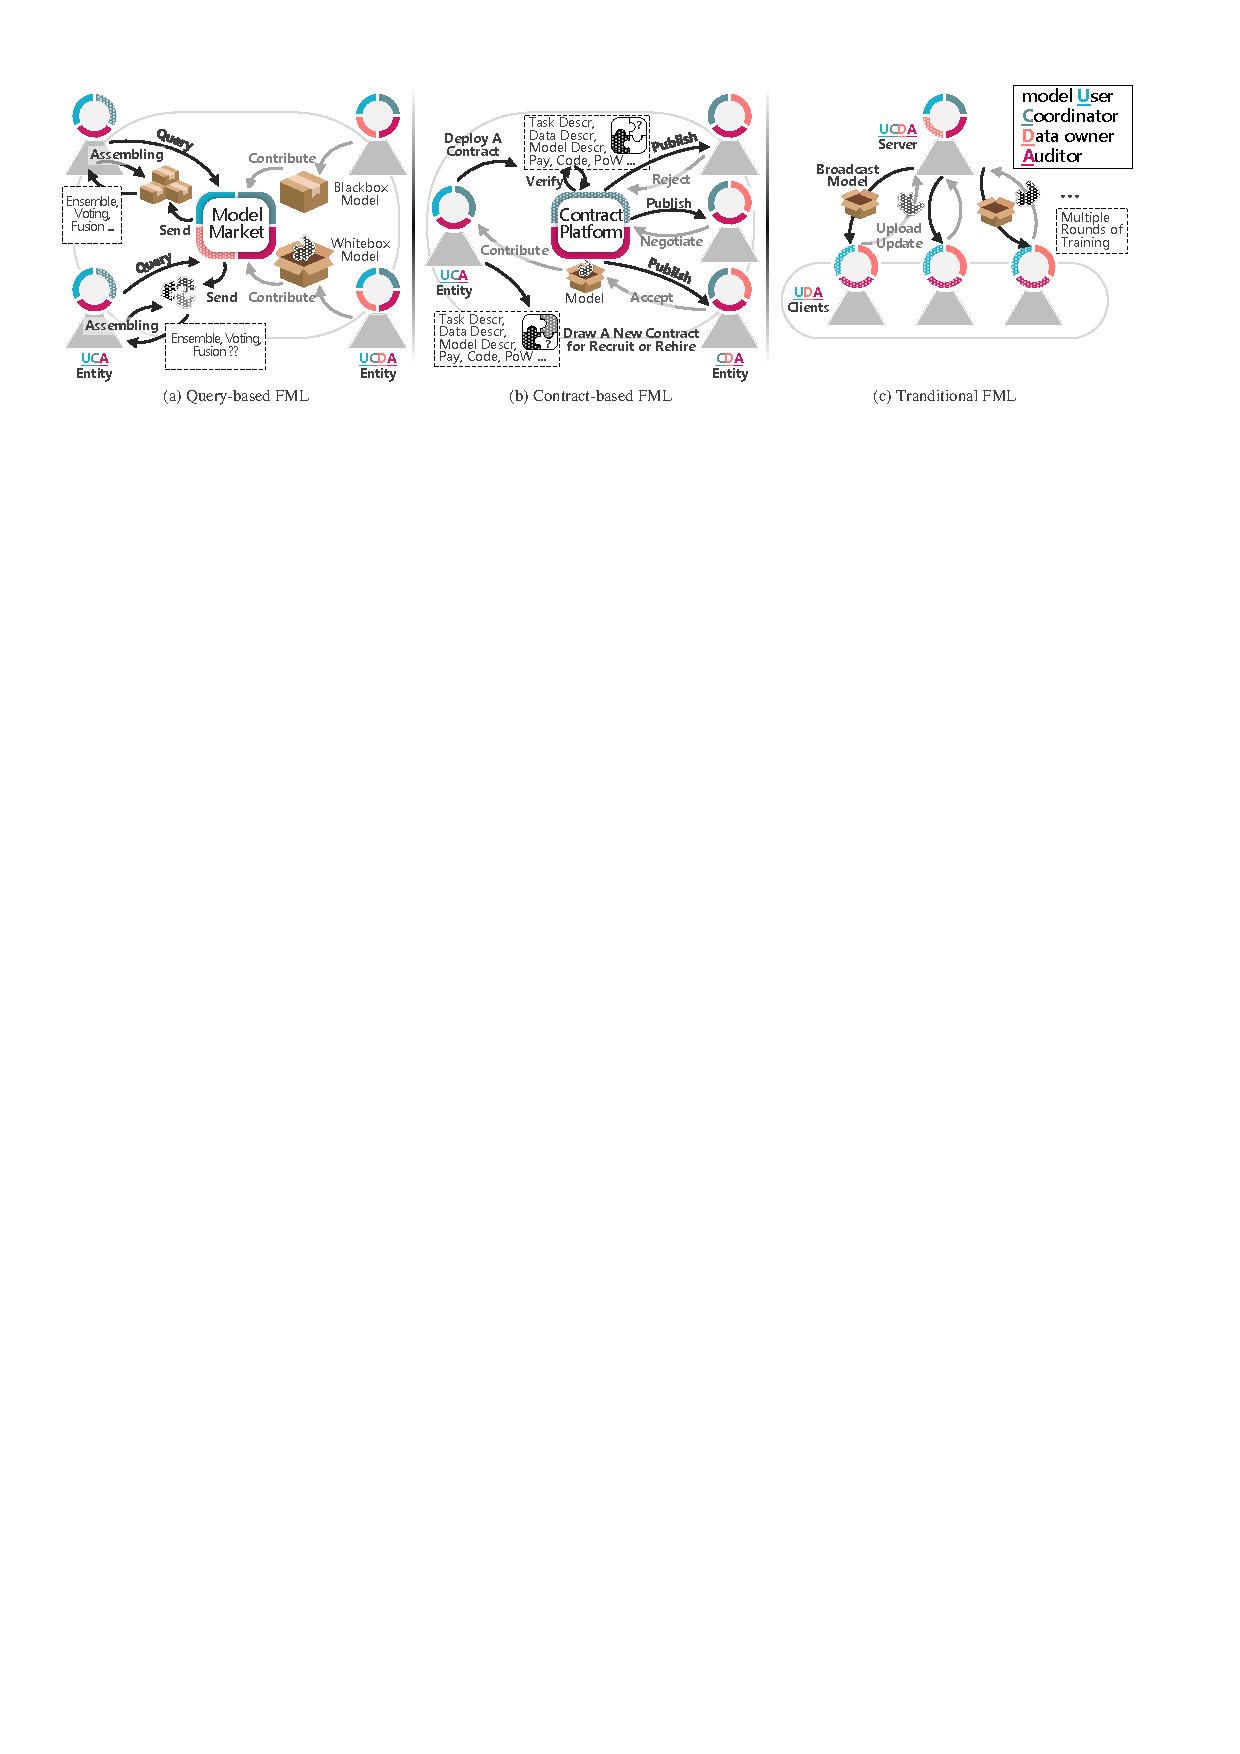
\includegraphics[width=\linewidth]{fig/coop_frame.pdf}
  \caption{Cooperation frameworks of FML.}
  \Description{}
\end{figure}

%%
%% The acknowledgments section is defined using the "acks" environment
%% (and NOT an unnumbered section). This ensures the proper
%% identification of the section in the article metadata, and the
%% consistent spelling of the heading.
\begin{acks}
ACK.
\end{acks}

%%
%% The next two lines define the bibliography style to be used, and
%% the bibliography file.
\bibliographystyle{ACM-Reference-Format}
\bibliography{REF}


%%
%% If your work has an appendix, this is the place to put it.
\appendix

\end{document}

\endinput
%%
%% End of file `sample-acmlarge.tex'.
